\documentclass[PI,LAB]{HSEUniversity}
% Возможные опции: KR или VKR; PI или BI
\usepackage{svg}
\usepackage{listings}

\title{Организация паттернов проектирования. Поведенческие  паттерны Интерпреатор и Наблюдатель}
\author{Виноградов Никита Андреевич}
\supervisor{к.т.н., доцент кафедры Информационных технологий в бизнесе НИУ ВШЭ-Пермь}{А.В.~Кычкин}

\Year{2020}


% Ссылка на файл с описание библиографии
\bibliography{library.bib}

%%%%%%%%%%%%%%%%%%%%%%%%%%%%%%%%
%%% ТЕКСТ РАБОТЫ %%%%%%%%%%%%%%%
\begin{document}

% Обязательные элементы оформления: заголовочный слайд, аннотация, оглавление
\maketitle


\chapter{Интерпретатор}
Поведенческий шаблон проектирования, решающий часто встречающуюся, но подверженную изменениям, задачу.
\section{Назначение}
\begin{itemize}
    \item Для заданного языка определяет представление его грамматики, а также интерпретатор предложений этого языка.
    \item Отображает проблемную область в язык, язык – в грамматику, а грамматику – в иерархии объектно-ориентированного проектировани.
\end{itemize}
\section{Структура}

\begin{FIGURE}[h]{Структура классов паттерна Заместитель\label{fig:example-figure}}
    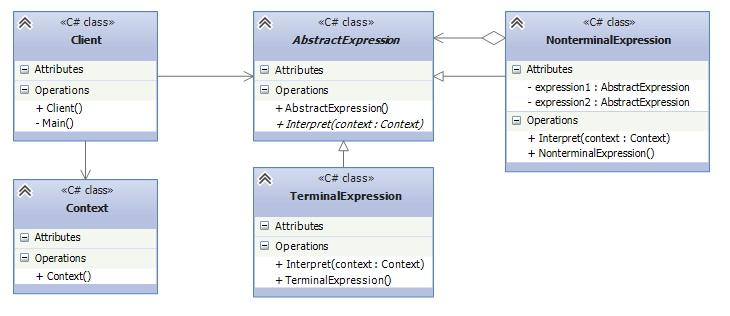
\includegraphics[width=1\textwidth]{../out/interpreter}
\end{FIGURE}

\textbf{Участники:}
\begin{itemize}
    \item \emph{AbstractExpression} - определяет интерфейс выражения, объявляет метод Interpret().
    \item \emph{TerminalExpression} - терминальное выражение, реализует метод Interpret() для терминальных символов грамматики. Для каждого символа грамматики создается свой объект TerminalExpression.
    \item \emph{NonterminalExpression} -  нетерминальное выражение, представляет правило грамматики. Для каждого отдельного правила грамматики создается свой объект NonterminalExpression.
    \item \emph{Context} - содержит общую для интерпретатора информацию. Может использоваться объектами терминальных и нетерминальных выражений для сохранения состояния операций и последующего доступа к сохраненному состоянию.
    \item \emph{Client} - строит предложения языка с данной грамматикой в виде абстрактного синтаксического дерева, узлами которого являются объекты TerminalExpression и NonterminalExpression.
\end{itemize}

\begin{FIGURE}[h]{Диаграмма последовательности паттерна Заместитель\label{fig:example-figure}}
    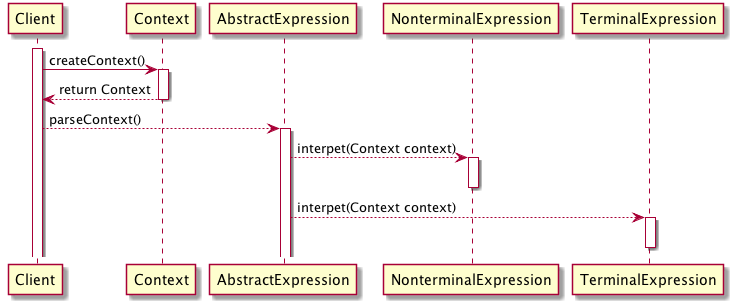
\includegraphics[width=1\textwidth]{../out/diagrams/interpreter/interpreter-default}
\end{FIGURE}

\section{Способ применения}
Пусть в некоторой, хорошо определенной области периодически случается некоторая проблема. Если эта область может быть описана некоторым “языком“, то проблема может быть легко решена с помощью “интерпретирующей машины“.
\chapter{Реализация паттернов}

\section{Диаграмма классов}
\begin{FIGURE}[h]{Диаграмма классов паттерна Интерпретатор\label{fig:example-figure}}
    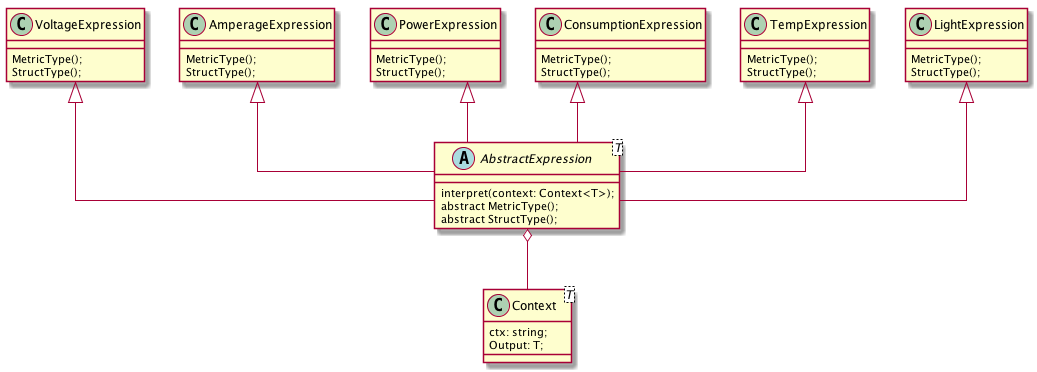
\includegraphics[width=1\textwidth]{../out/diagrams/interpreter-ts-class/interpreter-ts-class}
\end{FIGURE}
\emph{Участники:}
\begin{itemize}
    \item \emph{AbstractExpression} - определяет интерфейс выражения, объявляет метод Interpret().
    \item \emph{Context} - терминальное выражение, реализует метод Interpret() для терминальных символов грамматики. Для каждого символа грамматики создается свой объект.
    \item \emph{AmperageExpression} -  терминальное выражение, реализует метод Interpret() для терминальных символов грамматики. Для каждого символа грамматики создается свой объект.
    \item \emph{PowerExpression} - терминальное выражение, реализует метод Interpret() для терминальных символов грамматики. Для каждого символа грамматики создается свой объект.
    \item \emph{ConsumptionExpression} - терминальное выражение, реализует метод Interpret() для терминальных символов грамматики. Для каждого символа грамматики создается свой объект.
    \item \emph{LightExpression} - терминальное выражение, реализует метод Interpret() для терминальных символов грамматики. Для каждого символа грамматики создается свой объект.
    \item \emph{TempExpression} - терминальное выражение, реализует метод Interpret() для терминальных символов грамматики. Для каждого символа грамматики создается свой объект.
\end{itemize}
\pagebreak
\section{Диаграмма последовательности }

\begin{FIGURE}[h]{Диаграмма последовательности паттерна Интерпретатор\label{fig:example-figure}}
    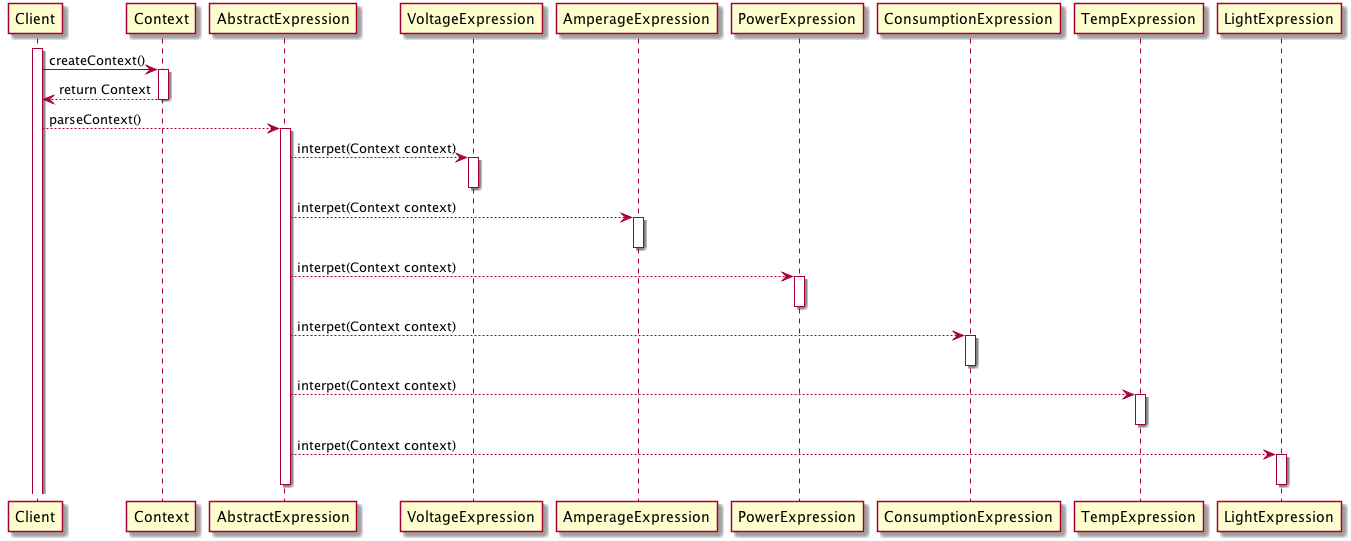
\includegraphics[width=1\textwidth]{../out/diagrams/interpreter-ts/interpreter-ts}
\end{FIGURE}
%%%%%%%%%%%%%%%%%%%%%%%%%%%%%%%%%%%%%%%%%%%
\chapter{Наблюдатель}
Это поведенческий паттерн проектирования, который создаёт механизм подписки, позволяющий одним объектам следить и реагировать на события, происходящие в других объектах.
\section{Назначение}
Паттерн Наблюдатель предлагает хранить внутри объекта издателя список ссылок на объекты подписчиков, причём издатель не должен вести список подписки самостоятельно. Он предоставит методы, с помощью которых подписчики могли бы добавлять или убирать себя из списка.
\section{Структура}

\begin{FIGURE}[h]{Структура классов паттерна Наблюдатель\label{fig:example-figure}}
    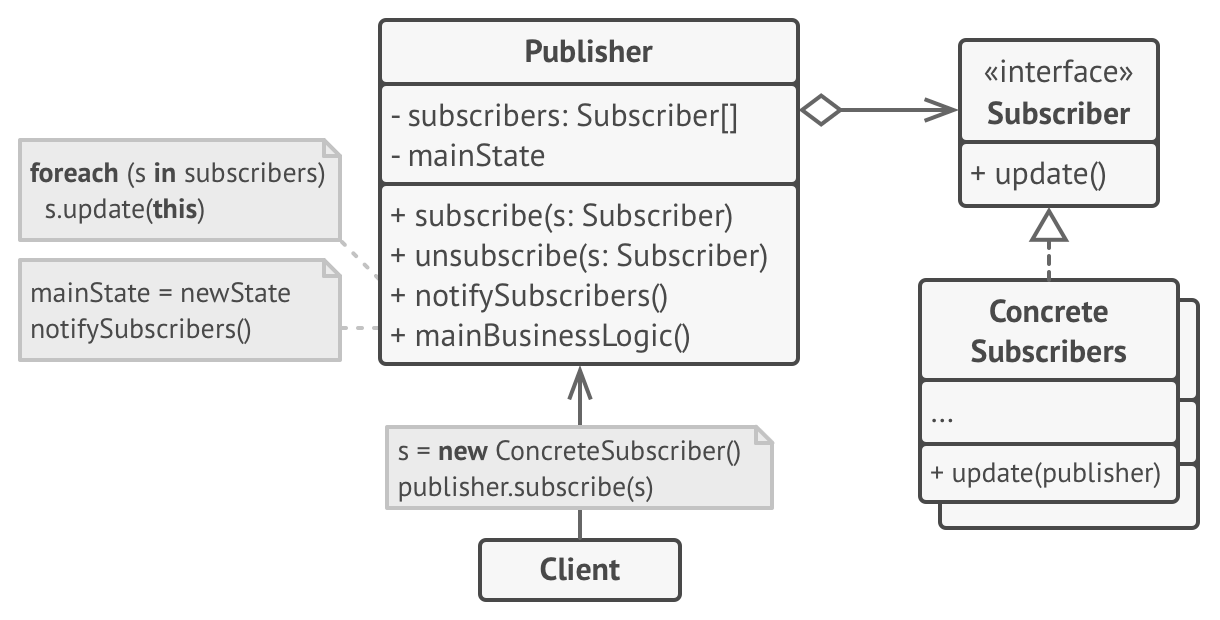
\includegraphics[width=1\textwidth]{../out/observer}
\end{FIGURE}

\textbf{Участники:}
\begin{itemize}
    \item \emph{Publisher} - Класс объекта который выполняет действия и оповещает наблюдателей.
    \item \emph{Subscriber} - определяет интерфейс для обновления отправителя.
    \item \emph{ConcreteSubscribers} - классы имплементирующие интерфейс Подписки и выполняют действия при обновлении.

\end{itemize}

\begin{FIGURE}[h]{Диаграмма последовательности паттерна Наблюдатель\label{fig:example-figure}}
    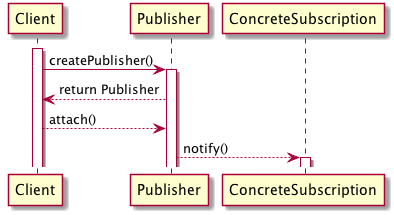
\includegraphics[width=0.7\textwidth]{../out/diagrams/observer/observer}
\end{FIGURE}

\section{Способ применения}
Когда после изменения состояния одного объекта требуется что-то сделать в других, но вы не знаете наперёд, какие именно объекты должны отреагировать.
\chapter{Реализация паттернов}

\section{Диаграмма классов}
\begin{FIGURE}[h]{Диаграмма классов паттерна Компоновщик\label{fig:example-figure}}
    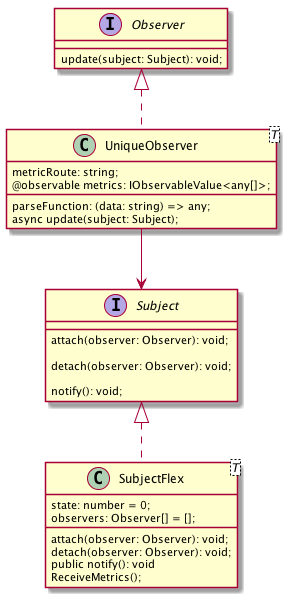
\includegraphics[width=0.3\textwidth]{../out/diagrams/observer-ts-class/observer-ts-class}
\end{FIGURE}
\emph{Участники:}
\begin{itemize}
    \item \emph{Observer} - Интерфейс объекта предоставляющий функции
    \item \emph{UniqueObserver} - определяет класс который будет прослушивать действия от субъекта
    \item \emph{Subject} - абстрактный класс задающий логику субъекта
    \item \emph{SubjectFlex} -  класс задающий массив объектов и предоставляет для уведомления
\end{itemize}
\pagebreak
\section{Диаграмма последовательности }

\begin{FIGURE}[h]{Диаграмма последовательности паттерна Компоновщик\label{fig:example-figure}}
    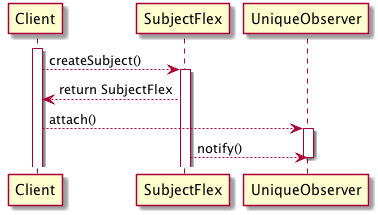
\includegraphics[width=0.7\textwidth]{../out/diagrams/observer-ts/observer-ts}
\end{FIGURE}


\section{Код программы}
\lstset{extendedchars=\true}
\begin{lstlisting}
    import {EletricMetric} from './electro';
    import {parseElectro, parseLight, parseTemp} from './sensor';
    import {action, computed, IObservableValue, observable} from 'mobx';
    
    interface Subject {
    attach(observer: Observer): void;
    
    detach(observer: Observer): void;
    
    notify(): void;
    }
    
    class SubjectFlex<T> implements Subject {
    
    public state: number = 0;
    
    private observers: Observer[] = [];
    
    public attach(observer: Observer): void {
    console.log('Subject: Attached an observer.');
    this.observers.push(observer);
    }
    
    public detach(observer: Observer): void {
    const observerIndex = this.observers.indexOf(observer);
    this.observers.splice(observerIndex, 1);
    console.log('Subject: Detached an observer.');
    }
    
    public notify(): void {
    console.log('Subject: Notifying observers...');
    for (const observer of this.observers) {
    observer.update(this);
    }
    }
    
    public async ReceiveMetrics() {
    this.notify();
    }
    }
    
    interface Observer {
    // Receive update from subject.
    update(subject: Subject): void;
    }
    
    export class UniqueObserver<T> implements Observer {
    metricRoute: string;
    @observable metrics: IObservableValue<any[]>;
    parseFunction: (data: string) => any;
    
    constructor(route: string, parseFunction: (data: string) => any) {
    this.metrics = observable.box([]);
    this.metricRoute = route;
    this.parseFunction = parseFunction;
    
    }
    
    @action
    public async update(subject: Subject) {
    fetch(`http://localhost:4000/${this.metricRoute}`, {
    method: 'GET',
    headers: {
    'Access-Control-Allow-Origin': '*',
    'Access-Control-Allow-Headers': '*'
    }
    }).then(item => item.json())
    .then(flex => this.metrics.set([...this.metrics.get(), this.parseFunction(flex.metric)]));
    }
    
    @computed get Metrics() {
    return this.metrics.get();
    }
    
    }
    
    
    export const electronic = new SubjectFlex<any>();
    
    export const electroObserve = new UniqueObserver<EletricMetric>('electro', parseElectro);
    export const tempObserve = new UniqueObserver<{ temp: number }>('temp', parseTemp);
    export const lightObserve = new UniqueObserver<{ lux: number }>('light', parseLight);
    //flex
    electronic.attach(electroObserve);
    electronic.attach(tempObserve);
    electronic.attach(lightObserve);
    
    
    
    import {EletricMetric} from './electro';
    
    class Context<T> {
    public ctx: string;
    public Output: T;
    
    constructor(ctx: string) {
    this.ctx = ctx;
    this.Output = <T> {};
    }
    
    }
    
    abstract class AbstractExpression<T> {
    
    public interpret = (context: Context<T>) => {
    if (context.ctx.length == 0) {
    return;
    }
    const idx = context.ctx.indexOf(this.MetricType());
    const data = context.ctx.split(this.MetricType());
    context.ctx = context.ctx.slice(idx + 1, context.ctx.length);
    context.Output[this.StructType()] = parseFloat(data[0]);
    console.log(context);
    };
    
    public abstract MetricType(): string;
    
    public abstract StructType(): string;
    }
    
    class VoltageExpression extends AbstractExpression<EletricMetric> {
    MetricType() {
    return 'V';
    }
    
    StructType() {
    return 'voltage';
    }
    }
    
    class AmperageExpression extends AbstractExpression<EletricMetric> {
    MetricType(): string {
    return 'A';
    }
    
    StructType(): string {
    return 'amperage';
    }
    
    }
    
    class PowerExpression extends AbstractExpression<EletricMetric> {
    MetricType(): string {
    return 'W';
    }
    
    StructType(): string {
    return 'power';
    }
    
    }
    
    class ConsumptionExpression extends AbstractExpression<EletricMetric> {
    MetricType(): string {
    return 'W';
    }
    
    StructType(): string {
    return 'consumption';
    }
    
    }
    
    class TempExpression extends AbstractExpression<{ temp: number }> {
    MetricType(): string {
    return 'C^';
    }
    
    StructType(): string {
    return 'temp';
    }
    
    }
    
    class LightExpression extends AbstractExpression<{ lux: number }> {
    MetricType(): string {
    return 'lux';
    }
    
    StructType(): string {
    return 'light';
    }
    
    }
    
    export const parseElectro = (data: string): any => {
    const ctx = new Context<EletricMetric>(data);
    const expArr = [
    new VoltageExpression(),
    new AmperageExpression(),
    new PowerExpression(),
    new ConsumptionExpression()
    ];
    expArr.forEach(item => item.interpret(ctx));
    return Dataframe(ctx.Output);
    };
    export const parseTemp = (data: string) => {
    const ctx = new Context<{ temp: number }>(data);
    const expArr = [
    new TempExpression()
    ];
    expArr.forEach(item => item.interpret(ctx));
    return FrameTemp(ctx.Output);
    };
    export const parseLight = (data: string) => {
    const ctx = new Context<{ lux: number }>(data);
    console.log('parse lux');
    const expArr = [
    new LightExpression()
    ];
    expArr.forEach(item => item.interpret(ctx));
    console.log(ctx);
    return FrameLux(ctx.Output);
    };
    
    const Dataframe = ({voltage, amperage, power, consumption}) =>
    ({
    name: generateData(), voltage, amperage, power, consumption
    });
    
    const FrameTemp = ({temp}) => ({
    name: generateData(), temp
    });
    const FrameLux = ({light}) => ({
    name: generateData(), lux: light
    });
    
    const generateData = () => {
    const data = new Date();
    return `${data.getMinutes()}:${data.getSeconds()}`;
    };
    
    
    
    \end{lstlisting}

\end{document}
